
%(BEGIN_QUESTION)
% Copyright 2009, Tony R. Kuphaldt, released under the Creative Commons Attribution License (v 1.0)
% This means you may do almost anything with this work of mine, so long as you give me proper credit

Suppose you walk up to this thermocouple, installed to measure the temperature of an enclosed process vessel, and connect a sensitive voltmeter to the terminals at the junction head:

$$\includegraphics[width=15.5cm]{i03972x01.eps}$$

Determine the process temperature if you read 7.825 millivolts with the voltmeter connected to the screw terminals inside the thermocouple head.  Assume a head temperature of 92 $^{o}$ F.

\vskip 10pt

Suppose at some later time you connected the voltmeter to the transmitter's input terminals and read 8.332 millivolts.  Calculate the process temperature at this time, assuming an ambient temperature of 66 $^{o}$F at the transmitter.  

\underbar{file i03972}
%(END_QUESTION)





%(BEGIN_ANSWER)



An equivalent circuit diagram shows the relationships between the thermocouple measurement junction (in the process), the two reference junctions formed where thermocouple wire meets copper wire, the digital multimeter, and the temperature transmitter (when the DMM is connected at the head):

$$\includegraphics[width=15.5cm]{i03972x02.eps}$$

$T_{process}$ = {\bf 388} deg F at 7.825 millivolts (measured at 92 $^{o}$F head)

\vskip 30pt

Another equivalent circuit diagram shows the relationships between the thermocouple measurement junction (in the process), the two reference junctions formed where thermocouple wire meets copper wire, the digital multimeter, and the temperature transmitter (when the DMM is connected at the transmitter):

$$\includegraphics[width=15.5cm]{i03972x03.eps}$$

$T_{process}$ = {\bf 385} deg F at 8.332 millivolts (measured at 66 $^{o}$F transmitter terminals)


%(END_ANSWER)





%(BEGIN_NOTES)

%INDEX% Measurement, temperature: thermocouple millivoltage interpretation

%(END_NOTES)


